\part{Axios}


\chapter{Overview}

Axios是一个基于Promise的用于浏览器和Node.js的HTTP客户端库。

\begin{compactitem}
\item Make XMLHttpRequests from the browser
\item Make http requests from node.js
\item Supports the Promise API
\item Intercept request and response
\item Transform request and response data
\item Cancel requests
\item Automatic transforms for JSON data
\item Client side support for protecting against XSRF
\end{compactitem}

Axios受到了Angularjs的\$http服务的启发,其目标是在Angularjs之外提供一个类似\$http的独立的服务。

Axios支持从浏览器中发出XMLHttpRequest请求,以及从Node.js发出HTTP请求。

Axios支持PromiseAPI,可以拦截请求和响应,转换请求和响应数据,以及取消请求等。

Axios可以自动转换JSON数据,以及在客户端防范XSRF攻击。

\begin{compactitem}
\item 使用NPM安装axios

\begin{lstlisting}[language=JavaScript]
$ npm install axios
\end{lstlisting}

\item 使用bower安装axios

\begin{lstlisting}[language=JavaScript]
$ bower install axios
\end{lstlisting}

\item 直接引入axios.js

\begin{lstlisting}[language=JavaScript]
<script src="https://unpkg.com/axios/dist/axios.min.js"></script>
\end{lstlisting}

\end{compactitem}

默认情况下,Axios会把Javascript对象序列化为JSON,可以通过如下的配置来使用application/x-www-form-urlencoded格式发送数据。

\section{Browser}

在浏览器中,可以使用URLSearchParams API来序列化为application/x-www-form-urlencoded格式:

\begin{lstlisting}[language=JavaScript]
var params = new URLSearchParams();
params.append('param1', 'value1');
params.append('param2', 'value2');
axios.post('/foo', params); 
\end{lstlisting}

URLSearchParams没有受到所有浏览器的支持,不过有一个polyfill可用(需要确保polyfill全局环境)。

qs库也可以用来序列化数据为application/x-www-form-urlencoded格式。

\begin{lstlisting}[language=JavaScript]
var qs = require('qs');
axios.post('/foo', qs.stringify({ 'bar': 123 }));
\end{lstlisting}

\section{Node.js}

Node.js的querystring模块支持application/x-www-form-urlencoded格式。



\begin{lstlisting}[language=JavaScript]
var querystring = require('querystring');
axios.post('http://something.com/', querystring.stringify({ foo: 'bar' });
\end{lstlisting}

Node.js也支持使用qs库来序列化数据为application/x-www-form-urlencoded格式。

\section{Semver}


\section{Promises}

axios取决于要支持的本地ES6 Promise实现。 如果当前环境不支持ES6 Promises,可以进行polyfill来实现支持。

\section{TypeScript}

Axios包含TypeScript定义。

\begin{lstlisting}[language=JavaScript]
import axios from 'axios';
axios.get('/user?ID=12345');
\end{lstlisting}


\begin{lstlisting}[language=JavaScript]

\end{lstlisting}




\begin{lstlisting}[language=JavaScript]

\end{lstlisting}




\begin{lstlisting}[language=JavaScript]

\end{lstlisting}





\begin{lstlisting}[language=JavaScript]

\end{lstlisting}

\chapter{Request}


\section{Request Aliases}

Axios为所有支持的请求方法提供了别名。

\begin{compactitem}
\item axios.request(config)
\item axios.get(url[,config])
\item axios.delete(url[,config])
\item axios.head(url[,config])
\item axios.post(url[,data[,config]])
\item axios.put(url[,data[,config]])
\item axios.patch(url[,data[,config]])
\end{compactitem}

当使用别名方法时,不需要在config中指定url,method和data属性。





\section{Single Request}


\subsection{GET}



\begin{lstlisting}[language=JavaScript]
// Make a request for a user with a given ID
axios.get('/user?ID=12345')
  .then(function(response){
      console.log(response);
  })
  .catch(function(error){
      console.log(error);
  });
\end{lstlisting}


下面的写法和上述GET请求的结果相同。



\begin{lstlisting}[language=JavaScript]
// Optionally the request above could also be done as
axios.get('/user',{
    params: {
       ID: 12345
    }
  })
  .then(function(response){
    console.log(response);
  })
  .catch(function(error){
    console.log(error);
  });
\end{lstlisting}


\subsection{POST}


\begin{lstlisting}[language=JavaScript]
axios.post('/user',{
     firstName: 'Fred',
     lastName: 'Flintstone'
   })
   .then(function(response){
      console.log(response);
   })
   .catch(function(error){
      console.log(error);
   });
\end{lstlisting}

\section{Multiple Request}


axios可以并发执行多个请求,例如:

\begin{lstlisting}[language=JavaScript]
function getUserAccount() {
   return axios.get('/user/12345/');
}

function getUserPermissions(){
   return axios.get('/user/12345/permissions');
}

axios.all([getUserAccount(),getUserPermissions()])
  .then(axios.spread(function(acct,perms){
     // Both requests are now complete
  }));
\end{lstlisting}




\chapter{Response}

\begin{figure}[htbp]
\centering
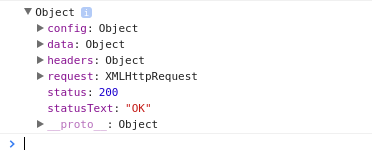
\includegraphics[scale=0.5]{axios-response.png}
\caption{Axios Response}
\end{figure}

\section{Response Schema}


Axios请求返回的响应包含的信息如下:



\begin{lstlisting}[language=JavaScript]
{
    // 'data' is the response that was provided by the server.
    data: {},
    
    // 'status' is the HTTP status code from the server response
    status: 200,
    
    // 'statusText' is the HTTP status message from the server response
    statusText: 'OK',
    
    // 'headers' the headers that the server responed with
    headers: {},
    
    // 'config' is the config that was provided to 'axios' for the request
    config: {}
}
\end{lstlisting}


\subsection{config}

\subsection{data}

\subsection{headers}

\subsection{request}


\subsection{status}


\subsection{statusText}


\subsection{\_\_proto\_\_}











\section{then}

如果使用then,可以以下面的方式来获取响应:

\begin{lstlisting}[language=JavaScript]
axios.get('/user/12345')
  .then(function(response){
     console.log(response.data);
     console.log(response.status);
     console.log(response.statusText);
     console.log(response.headers);
     console.log(response.config);
  });
\end{lstlisting}




\section{catch}

如果使用catch或传递一个抑制回调(rejection callback)作为then的第二个参数,那么可以通过error对象来获取和处理响应错误。

\begin{lstlisting}[language=JavaScript]
axios.get('/user/12345')
  .then(function(response){
     console.log(response.data);
     console.log(response.status);
     console.log(response.statusText);
     console.log(response.headers);
     console.log(response.config);
  })
  .catch(function(error){
     if(error.response){
         // The request was made, but the server responed with a status code
         // that falls out of the range of 2xx
         console.log(error.response.data);
         console.log(error.response.status);
         console.log(error.response.statusText);
         console.log(error.response.headers);
     }else{
         // Something happened in setting up the request that triggered an error
         console.log('Error',error.message);
     }
     console.log(error.config);
  });
\end{lstlisting}


\chapter{Error}



\begin{lstlisting}[language=JavaScript]
axios.get('/user/12345')
  .catch(function (error) {
    if (error.response) {
      // The request was made, but the server responded with a status code
      // that falls out of the range of 2xx
      console.log(error.response.data);
      console.log(error.response.status);
      console.log(error.response.headers);
    } else {
      // Something happened in setting up the request that triggered an Error
      console.log('Error', error.message);
    }
    console.log(error.config);
  });
\end{lstlisting}

axios允许使用validateStatus定义一个自定义HTTP状态码来表示错误范围。例如,下面的示例中,当状态代码大于或等于500时,axios就拦截结果并拒绝访问。

\begin{lstlisting}[language=JavaScript]
axios.get('/user/12345',{
      validateStatus: function(status){
          return statue < 500; // Reject only if the status code is greater than or equal to 500
      }
   })
\end{lstlisting}






\begin{lstlisting}[language=JavaScript]

\end{lstlisting}



\begin{lstlisting}[language=JavaScript]

\end{lstlisting}




\chapter{Configure}


Axios的配置项将与优先顺序合并,首先是在lib/defaults.js中配置的默认值,然后是实例的defaults属性,最后是请求的config参数,其中后者将优先于前者。 


\begin{lstlisting}[language=JavaScript]
// Create an instance using the config defaults provided by the library
// At this point the timeout config value is `0` as is the default for the library
var instance = axios.create();

// Override timeout default for the library
// Now all requests will wait 2.5 seconds before timing out
instance.defaults.timeout = 2500;

// Override timeout for this request as it's known to take a long time
instance.get('/longRequest', {
  timeout: 5000
});
\end{lstlisting}


\section{Default Config}

Axios允许指定默认的配置来应用到每一个请求中。

\subsection{Global Config}



\begin{lstlisting}[language=JavaScript]
axios.defaults.baseURL = 'http://api.example.com';
axios.defaults.headers.common['Authorization'] = AUTH_TOKEN;
axios.defaults.headers.post['Content-Type'] = 'application/x-www-form-urlencoded';
\end{lstlisting}

\subsection{Instance Config}





\begin{lstlisting}[language=JavaScript]
// Set config defaults when creating the instance
var instance = axios.create({
   baseURL: 'https://api.example.com'
});

// Alter defaults after instance has been created
instance.defaults.headers.common['Authorization'] = AUTH_TOKEN;
\end{lstlisting}




\section{Relevent Config}


axios允许通过将相关配置传递给axios来进行请求。

\subsection{axios(config)}


\begin{lstlisting}[language=JavaScript]
// send a POST request
axios({
   method: 'post',
   url: '/user/12345',
   data: {
      firstName: 'Fred',
      lastName: 'Flintstone'
   }
});
\end{lstlisting}

\subsection{axios(url[,config])}



\begin{lstlisting}[language=JavaScript]
// send a GET request(default method)
axios('/user/12345');
\end{lstlisting}

\section{Custom Config}

Axios支持使用自定义配置来创建Axios的新实例。

\subsection{axios.create([config])}



\begin{lstlisting}[language=JavaScript]
var instance = axios.create({
   baseURL: 'https://some-domain.com/api',
   timeout: 1000,
   headers: {
       'X-Custom-Header': 'foobar'
   }
});
\end{lstlisting}

用户指定的配置将与实例配置合并。

\chapter{Cutomization}

\section{Instance Method}


下面列出了可用的实例方法。 

\begin{compactitem}
\item axios\#request(config)
\item axios\#get(url[,config])
\item axios\#delete(url[,config])
\item axios\#head(url[,config])
\item axios\#post(url[,data[,config]])
\item axios\#put(url[,data[,config]])
\item axios\#patch(url[,data[,config]])
\end{compactitem}






\subsection{get}


\subsection{put}




\subsection{post}





\subsection{head}


\subsection{patch}


\subsection{delete}


\subsection{request}





\section{Instance Configure}

Axios用于发出请求的可用配置选项中,只有url是必需的。 如果未指定方法,请求将默认为GET。

\begin{lstlisting}[language=JavaScript]
{
   // 'url' is the server URL that will be used for the request
   url: '/user',
   
   // 'method' is the request method to be used when making the request
   method: 'get', // default
   
   // 'baseURL' will be prepended to 'url' unless 'url' is absolute.
   // It can be convenient to set 'baseURL' for an instance of axios to pass relative URLs
   // to methods of that instance
   baseURL: 'https://some-domain.com/api/',
   
   // 'transformRequest' allows change to the request data before it is sent to the server
   // This is only applicable for request method 'PUT','POST' and 'PATCH'.
   // The last function in the array must return a string, an ArrayBuffer, or a Stream
   transformRequest: [function(data){
      // Do whatever you want to transform the data
      return data;
   }]
   
   // 'transformResponse' allows changes to the response data to be made before 
   // it is passed to then/catch
   transformResponse: [function(data){
      // Do whatever you want to transform the data
      return data;
   }]
   
   // 'headers' are custom headers to be sent
   headers: {
     'X-Requested-With': XMLHttpRequest'
   }
   
   // 'params' are the URL parameters to be sent with the request
   // Must be a plain object or a URLSearchParams object
   params: {
      ID: 12345
   }
   
   // 'paramsSerializer' is optional function in charge of serializing 'params'
   // (e.g. https://www.npmjs.com/package/qs, http://api.jquery.com/jquery.param/)
   paramsSerializer: function(params){
      return Qs.stringify(params,{arrayFormat: 'brackets'})
   }
   
   // 'data' is the data to be sent as the request body.
   // Only application for request methods 'PUT','POST', and 'PATCH'.
   // When no 'transformRequest' is set,must be of one of the following type:
   // - string, plain object, ArrayBuffer, ArrayBufferView,URLSearchParams
   // - Browser only: FormData, File, Blob
   // - Node only: Stream
   data: {
       firstName: 'Fred'
   }
   
   // 'timeout' specifies the number of milliseconds before the request times out.
   // If the request takes longer than 'timeout', the request will be aborted.
   timeout: 1000,
   
   // 'withCredentials' indicates whether or not cross-site Access-Control requests
   // should be made using credentials
   withCredentials: false,//default
   
   // 'adapter' allows custom handling of requests which makes testing easier.
   // Return a promise and supply a valid response.
   adapter: function(config){
      /* ... */
   },
   
   // 'auth' indicates that HTTP Basic auth should be used, and supplies credentials.
   // This will set an 'Authorization' header, overwriting any existing
   // 'Authorization' custom headers you have set using 'headers'.
   auth: {
       username: 'janedoe',
       password: 's00pers3cret'
   },
   
   // 'responseType' indicates the type of data that the server will respond with 
   // options are 'arraybuffer','blob','document','json','text','stream'.
   responseType: 'json',// default
   
   // 'xsrfCookieName' is the name of the cookie to use as a value for xsrf token
   xsrfCookieName: 'XSRF-TOKEN',//default
   
   // 'xsrfHeaderName' is the name of the http header that carries the xsrf token value
   xsrfHeaderName: 'X-XSRF-TOKEN', //default
   
   // 'onUploadProgress' allows handling of progress events for uploads
   onUploadProgress: function(progressEvent){
      // Do whatever you want with the native progress event
   },
   
   // 'onDownloadProgress' allow handling of progress events for downloads
   onDownloadProgress: function(progressEvent){
      // Do whatever you want with the native progress event
   },
   
   // 'maxContentLength' defines the max size of the http response content allowed
   maxContentLength: 2000,
   
   // 'validateStatus' defines whether to resolve or reject the promise for a given 
   // HTTP response status code. If 'validateStatus' returns 'true' (or is set to 'null' 
   // or 'undefined'), the promise will be resolved; otherwise, the promise will be rejected.
   'validateStatus': function(status){
       // return status >= 200 && status < 300; //default
   },
   
   // 'maxRedirects' defines the maximum number of redirects to follow in node.js.
   // If set to 0, no redirects will be followed.
   maxRedirects: 5,
   
   // 'httpAgent' and 'httpsAgent' defines a custom agent to be used when performing http 
   //  and https requests, respectively, in node.js. This allows to configure options like
   // 'keepAlive' that are not enabled by default.
   httpAgent: new http.Agent({keepAlive: true}),
   httpsAgent: new https.Agent({keepAlive: true}),
   
   // 'proxy' defines the hostname and port of the proxy server
   // 'auth' indicates that HTTP Basic auth should be used to connect to the proxy, 
   // and supplies credentials.
   // This will set an 'Proxy-Authorization' header, overwriting any existing 'Proxy-Authorization' 
   // custom headers you have set using 'headers'.
   proxy: {
      host: 127.0.0.1,
      port: 9000,
      auth: {
          username: 'mikeymike',
          password: 'rapunz31'
      }
   },
   
   // 'cancelToken' specifies a cancel token that can be used to cancel the request
   cancelToken: new CancelToken(function(cancel){})
}
\end{lstlisting}

\subsection{url}


\subsection{method}


\subsection{baseURL}


\subsection{transformRequest}


\subsection{transformResponse}



\subsection{headers}



\subsection{params}


\subsection{paramsSerializer}


\subsection{data}


\subsection{timeout}

\subsection{withCredentials}


\subsection{adapter}

\subsection{adapter}


\subsection{auth}


\subsection{responseType}


\subsection{xsrfCookieName}


\subsection{xsrfHeaderName}

\subsection{onUploadProgress}


\subsection{onDownloadProgress}

\subsection{maxContentLenght}


\subsection{validateStatus}


\subsection{maxRedirects}


\subsection{httpAgent}


\subsection{httpsAgent}


\subsection{proxy}


\subsection{cancelToken}










\chapter{Cancellation}

Axios的cancel token API基于cancelable promises proposal。


Axios支持使用cancel token来取消请求,而且Axios支持使用相同的cancel token取消多个请求。



可以使用Axios的CancelToken.source工厂来创建cancel token:




\begin{lstlisting}[language=JavaScript]
var CancelToken = axios.CancelToken;
var source = CancelToken.source();

axios.get('/user/12345', {
  cancelToken: source.token
}).catch(function(thrown) {
  if (axios.isCancel(thrown)) {
    console.log('Request canceled', thrown.message);
  } else {
    // handle error
  }
});

// cancel the request (the message parameter is optional)
source.cancel('Operation canceled by the user.');
\end{lstlisting}


也可以通过将执行器函数传递给CancelToken构造函数来创建cancel token:

\begin{lstlisting}[language=JavaScript]
var CancelToken = axios.CancelToken;
var cancel;

axios.get('/user/12345', {
  cancelToken: new CancelToken(function executor(c) {
    // An executor function receives a cancel function as a parameter
    cancel = c;
  })
});

// cancel the request
cancel();
\end{lstlisting}





\chapter{Concurrency}


Axios提供了相应的辅助函数来处理并发请求。

\section{axios.all(iterable)}



\section{axios.spread(callback)}


\chapter{Interceptor}


Axios的请求或响应数据在被最终处理之前可以使用then和catch拦截器来拦截,而且用户还可以移除拦截器。



\begin{lstlisting}[language=JavaScript]
var myInterceptor = axios.interceptors.request.use(function () {/*...*/});
axios.interceptors.request.eject(myInterceptor);
\end{lstlisting}

Axios允许在自定义axios实例上添加拦截器。

\begin{lstlisting}[language=JavaScript]
var instance = axios.create();
instance.interceptors.request.use(function () {/*...*/});
\end{lstlisting}

\section{Request Interceptor}



\begin{lstlisting}[language=JavaScript]
// Add a request interceptor
axios.interceptors.request.use(function (config) {
    // Do something before request is sent
    return config;
  }, function (error) {
    // Do something with request error
    return Promise.reject(error);
  });
\end{lstlisting}

\section{Reponse Interceptor}


\begin{lstlisting}[language=JavaScript]
// Add a response interceptor
axios.interceptors.response.use(function (response) {
    // Do something with response data
    return response;
  }, function (error) {
    // Do something with response error
    return Promise.reject(error);
  });
\end{lstlisting}






\begin{lstlisting}[language=JavaScript]

\end{lstlisting}




\begin{lstlisting}[language=JavaScript]

\end{lstlisting}




\begin{lstlisting}[language=JavaScript]

\end{lstlisting}



\begin{lstlisting}[language=JavaScript]

\end{lstlisting}



\begin{lstlisting}[language=JavaScript]

\end{lstlisting}




\begin{lstlisting}[language=JavaScript]

\end{lstlisting}



\begin{lstlisting}[language=JavaScript]

\end{lstlisting}



\begin{lstlisting}[language=JavaScript]

\end{lstlisting}




\begin{lstlisting}[language=JavaScript]

\end{lstlisting}



\begin{lstlisting}[language=JavaScript]

\end{lstlisting}



\begin{lstlisting}[language=JavaScript]

\end{lstlisting}



\begin{lstlisting}[language=JavaScript]

\end{lstlisting}




\begin{lstlisting}[language=JavaScript]

\end{lstlisting}



\begin{lstlisting}[language=JavaScript]

\end{lstlisting}



\begin{lstlisting}[language=JavaScript]

\end{lstlisting}




\begin{lstlisting}[language=JavaScript]

\end{lstlisting}




\begin{lstlisting}[language=JavaScript]

\end{lstlisting}



\begin{lstlisting}[language=JavaScript]

\end{lstlisting}



\begin{lstlisting}[language=JavaScript]

\end{lstlisting}




\begin{lstlisting}[language=JavaScript]

\end{lstlisting}



\begin{lstlisting}[language=JavaScript]

\end{lstlisting}



\begin{lstlisting}[language=JavaScript]

\end{lstlisting}




\begin{lstlisting}[language=JavaScript]

\end{lstlisting}





\begin{lstlisting}[language=JavaScript]

\end{lstlisting}



\begin{lstlisting}[language=JavaScript]

\end{lstlisting}



\begin{lstlisting}[language=JavaScript]

\end{lstlisting}




\begin{lstlisting}[language=JavaScript]

\end{lstlisting}



\begin{lstlisting}[language=JavaScript]

\end{lstlisting}



\begin{lstlisting}[language=JavaScript]

\end{lstlisting}




\begin{lstlisting}[language=JavaScript]

\end{lstlisting}




\begin{lstlisting}[language=JavaScript]

\end{lstlisting}



\begin{lstlisting}[language=JavaScript]

\end{lstlisting}



\begin{lstlisting}[language=JavaScript]

\end{lstlisting}




\begin{lstlisting}[language=JavaScript]

\end{lstlisting}



\begin{lstlisting}[language=JavaScript]

\end{lstlisting}



\begin{lstlisting}[language=JavaScript]

\end{lstlisting}




\begin{lstlisting}[language=JavaScript]

\end{lstlisting}